\chapter{使用蒙特卡洛方法进行探测器背景模拟}
\label{chapter:background}

PandaXIII 实验需要着重解决的问题之一便是构建极低背景的探测环境,因此我们需要大量的数据来支持探测器设计及材料筛选。为了能够在实际建造探测器前得到相应的数据,我们使用Geant4\supercite{Agostinelli:2002hh}蒙特卡洛模拟框架构建了整个探测器的模型,并用它模拟得到了探测器不同组件以及环境对实验本底的贡献。本章详细描述了该模拟工作的细节以及得到的结果。

\section{模拟中目标元素及所使用的工具}

 TPC 探测器主体由一个相对较厚的铜罐构成,因其屏蔽效应外部的 $\alpha$ 射线和 $\beta$ 射线并不能穿透罐体进入探测器内部,所以实验的本底辐射主要来自于探测器铜罐内部各个元器件的辐射以及环境和材料中的 $\gamma$ 射线。

实验中我们定义 $^{136}$Xe NLDBD 衰变总能量附近的区域($Q_{\beta\beta}-2\sigma$ , $Q_{\beta\beta}+2\sigma$)为能量敏感区域(Region Of Interest, ROI),其中 $Q_{\beta\beta}=2458$keV ,$\sigma$ 为探测器在 $Q_{\beta\beta}$ 处的绝对能量分辨率,即探测器设计中的 3\% FWHW(半高全宽)。通过计算可以得到 ROI 范围为 2395keV 到 2520keV。根据各种放射性元素的衰变能量和在自然界中的丰度,结合既往有关 $^{136}$Xe NLDBD 实验研究结果,我们可以得到本底辐射主要来自于 $^{214}$Bi 的 2447.8keV $\gamma$ 衰变以及 $^{208}$Tl  2614.5keV 的$\gamma$ 衰变。这两种放射性同位素位于 \utte 和 \thttt 的衰变链中,因此他们广泛分布于各种生产生活材料中,成为了 PandaXIII 背景模拟中所着重关注的目标元素。

除了 $^{214}$Bi 和 $^{208}$Tl 这两种同位素之外,\cose 也需要被关注。它会释放出 1.33MeV 和 1.17MeV 两种 $\gamma$ 射线,其能量和也恰巧落在了 ROI 中。但是这两个 $\gamma$ 射线之间相对独立,它们同时被探测器探测到(这是一个符合事件)的概率很小。因此在后续模拟中 \cose 并未被着重研究。综合而言,PandaXIII 背景模拟中所关注的元素便是 \utte 和 \thttt 以及 \cose  , 表\ref{tab:activities}给出了构建探测器的原料中这些元素的放射性活度。

\renewcommand\arraystretch{1.4}
\begin{table*}[tbh]
    \centering
    \begin{tabular*}{0.75\textwidth}{@{\extracolsep{\fill}}cccc}
        \hline
        \hline
        \multirow{2}{*}{\textbf{材料}} & \multicolumn{3}{c}{\textbf{放射性活度 ($\mu$Bq/kg)}}\\
            & $^{232}$Th & $^{238}$U  & $^{60}$Co \\ \hline
        铜      & 0.2        &   0.75     &     100     \\
        PTFE    & 0.1        &   4.94      &    -      \\
        不锈钢  & 0.32$\times$10$^3$          &    0.5$\times$10$^3$      &     2.6$\times$10$^3$     \\
        超纯水  & 0.04          &     0.12      &     -     \\
        混泥土  & 9.9$\times$10$^6$          &    4.4$\times$10$^6$   &    -    \\
        \hline
        \hline
    \end{tabular*}
    \caption{构建探测器所用材料中不同放射性元素活度表。铜和PTFE的活动数据来自于文献\cite{Abgrall:2016cct},不锈钢的数据来自于文献\cite{LZ_CDR},超纯水的数据来自于PandaXIII的中期报告\cite{cdr},混泥土的数据来自于文献\cite{Zeng2014}。}
    \label{tab:activities}
  \end{table*}
  

PandaXIII 模拟工作中我们使用了 Geant4 作为蒙特卡洛模拟框架。 Geant4 是由 CERN 开发基于 C++ 的蒙特卡罗应用包,主要用于模拟追踪粒子在物质中所发生的各种物理过程。它实现了完成蒙特卡洛模拟所需要的各种方法:包括径迹追踪,探测器几何构建,物理过程的处理以及散射截面数据等等。Geant4 中内置的物理过程包含了大能量尺度下诸多粒子与物质间的相互作用,所以该软件被广泛的应用在了核物理,高能物理,医学研究等领域。

我们在 Geant4 软件框架的基础上二次开发了两组软件以满足 PandaXIII 实验模拟的需求,它们分别被称作 BambooMC 和 RestG4 。BambooMC 是基于 PandaX 二期工作(暗物质探测,PandaXII)的模拟需求开发改进而成,并被良好的应用在了 PandaXIII 三期项目中。RestG4 则是基于 REST \supercite{tomas2013development} 软件包构建的一个模块。PandaXIII 实验使用这两种框架独立进行了背景模拟工作,并对两者的结果进行了交叉检查以确保结果的正确性。本文中的模拟工作都是由 BambooMC 模拟框架完成。

\section{探测器模型及组件中的本底来源}

\begin{figure}[tbh]
    \centering
    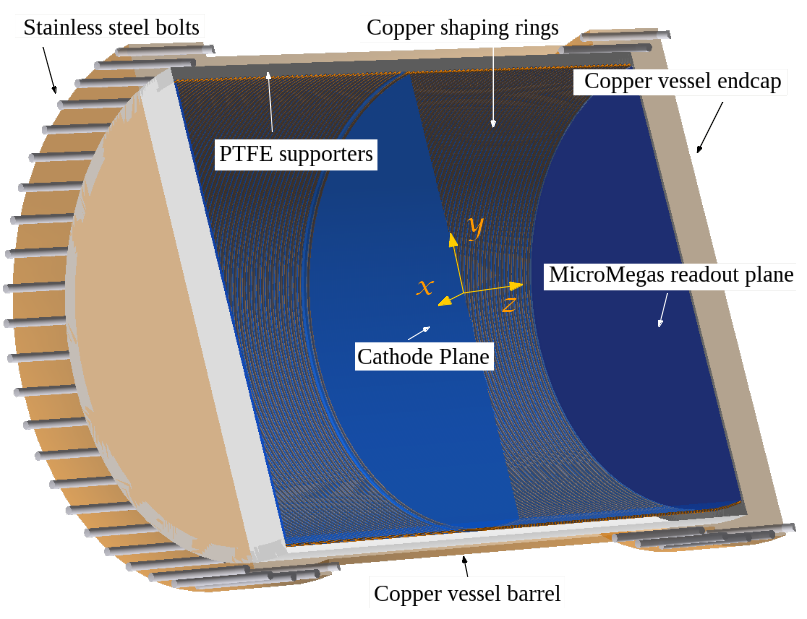
\includegraphics[width=0.4\columnwidth]{pic/fig3.png}
    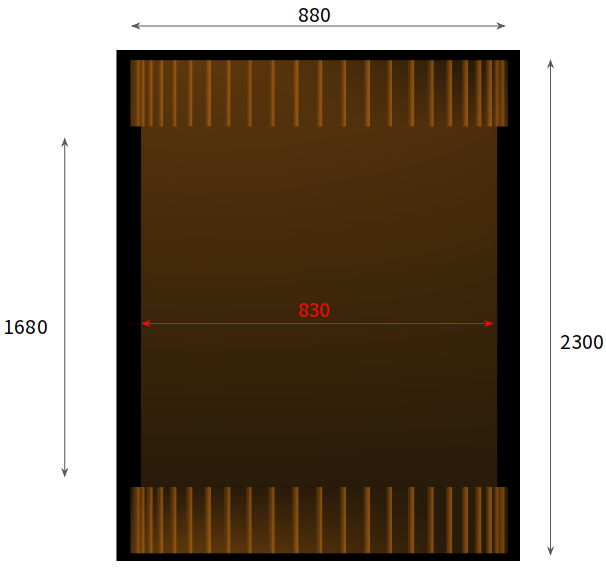
\includegraphics[width=0.4\columnwidth]{pic/fig5.png}
    \caption{左图:由 BambooMC 构建的 PandaXIII 探测器模型剖面示意图。右图:探测器铜罐正视图。}
    \label{fig:detector_bamboomc}
\end{figure}

我们使用 BambooMC 构建出的探测器模型如图\ref{fig:detector_bamboomc}所示。探测器主体是一个由有法兰的罐体和两端端盖组成的铜制压力容器,端盖和罐体之间使用 96 个不锈钢螺钉铆和,罐体厚度为 3 厘米,端盖厚度为 15 厘米。铜罐内部便是时间漂移室,它使用 5 厘米厚的空心柱形 PTFE 材料作为支撑结构,延 Z 方向(铜罐对称轴方向)镶嵌 99 个管状铜环,和读出平面以及极板一起组成场笼,用于形成Z方向上的漂移电场。两个 MM 组成的读出平面放置与铜罐内部两端,铜罐中心圆形极板将探测器分为上下两个漂移室。上述原件的主要尺寸如表\ref{tab:parameters_geometry}所示。我们在铜罐内填充了200kg 10bar 压强的 Xe+1\%TMA 混合气体,并将探测器放置于中国锦屏地下实验室所建造的超纯水水池中。

\begin{table*}[thb]
    \begin{center}
        \begin{tabular*}{0.75\textwidth}{@{\extracolsep{\fill}}ccccc}
        \hline
        \hline
        \textbf{组件} & \textbf{参数} & \textbf{值} & \textbf{材料} & \textbf{质量} \\ \hline
        \multirow{3}{*}{铜罐罐体} 
            & 内径 & 80\,cm & \multirow{3}{*}{铜} & \multirow{3}{*}{3438 kg} \\
            & 高度 & 200\,cm &  &    \\   
            & 壁厚 & 3\,cm &  &    \\\hline
        \multirow{2}{*}{铜罐端盖} 
            & 直径 & 88\,cm & \multirow{2}{*}{铜} & \multirow{2}{*}{3320 kg} \\
            & 厚度 & 15\,cm &  &    \\\hline
        \multirow{2}{*}{螺钉} 
            & 直径 & 1.4\,cm & \multirow{2}{*}{不锈钢} & \multirow{2}{*}{230.1 kg} \\
            & 高度 & 40\,cm &  &    \\\hline
        \multirow{4}{*}{场笼} 
            & 内径 & 75\,cm & \multirow{3}{*}{PTFE} & \multirow{3}{*}{1042 kg} \\
            & 高度 & 200\,cm &  & \\ 
            & 厚度 & 5\,cm &  & \\ 
            & 铜环个数 & 99 &    \multirow{1}{*}{铜}  & 118.2 kg \\\hline
        中心极板 
            & 厚度   &   50\,$\mu$m     &   \multirow{1}{*}{铜}  &    0.79 kg   \\   
        \hline
        \hline
        \end{tabular*}
        \caption{探测器主要元件的几何参数,组成材料以及质量数据表。\supercite{cdr}}
        \label{tab:parameters_geometry}
    \end{center}
\end{table*}
  
下述列表详细描述了在探测器背景模拟过程中,我们对于探测器各个组件及周围环境的处理细节:
\vspace{0.4cm}

\begin{description}

    \item[铜罐] 模拟中我们将罐体和端盖组成的压力铜罐容器整体作为研究对象。如表\ref{tab:activities}所示,虽然无氧铜可以做到比较洁净(radiopure),但是铜罐作为接近探测气体中质量最大的组件,还是可能会对本底做出较大贡献。

    \item[电子学] 因为大量电气元件的存在,探测器电子学部分不能做到相对洁净,所以在探测器设计中它被放在了 15 厘米厚的铜罐端盖的外侧以降低其本底贡献。模拟中我们认为电子学部分 $^{238}$U 和 $^{232}$Th 活度分别为 0.26Bq 和 0.07Bq。这项数据来自于 PandaX 二期暗物质实验中的相关研究。
    
    \item[场笼] 场笼是由 5 厘米厚 PTFE 支撑结构以及等距嵌入的铜环组成,它是探测器中质量仅次于铜罐的组件。模拟中使用的相关数据如表\ref{tab:activities}所示。

    \item[不锈钢螺钉] 在铆合铜罐时我们使用了96个不锈钢螺丝钉。从表\ref{tab:activities}可以看出不锈钢的放射性洁净程度远远低于其它低本底材料,其含有的 \utte 和 \thttt 活度比铜高了3个量级。因此虽然螺钉的整体质量相对较小,它对本底依然可能造成很大的影响。模拟中不锈钢螺钉被简化为圆柱体以加速模拟的进行。

    \item[水池中的水] 因为超纯水放射性相对较低,并且有自屏蔽效应,所以我们在模拟中只考虑了TPC周围5米范围内水中发生的衰变事件。

    \item[实验室水泥墙壁] 从表\ref{tab:activities}来看水泥的放射性远远高于其他材料。虽然超纯水池能够屏蔽绝大部分来自于水泥墙壁的本地,但我们依然需要通过模拟给出具体的数值以指导水池尺寸设计。同时因为水池屏蔽效应的存在,如果直接模拟墙壁中 $^{238}$U 和 $^{232}$Th 的衰变,那么因为模拟效率和模拟数量的限制,基本上不可能有射线能够穿过水池到达探测器,所以我们使用了下列的方式来估计实验室水泥墙壁的本底贡献:

    \begin{itemize}
        \item 第一步,我们模拟得到了在一块巨大的水泥块表面水泥内部 $^{238}$U 和 $^{232}$Th 产生的 $\gamma$ 射线流的能谱。
        \item 第二步,我们将整个水池分为若干层,逐层的模拟。根据上一步模拟得到的 $\gamma$ 能谱信息,在第一层水的外表面均匀放置$\gamma$粒子,模拟得到穿过这一层水达到内表面的 $\gamma$ 粒子能谱,方向分布以及数目信息。然后在第二层的外表面根据第一层得到的粒子能谱和方向分布放置 $\gamma$ 粒子,重复上述模拟过程。假设在第 $i$ 层模拟了 $N_i$ 个$\gamma$ 粒子,只有 $n_i$ 个穿过了水池被记录下来(这里显然 $n_i<<N_i$),我们定义 $\alpha_i=N_{i+1}/n_i$ 为放大系数,那么在最后一层模拟得到的结果等价于不分层直接模拟 $$N_{eq}=N_0\prod_{i=1}^{t}a_i$$ 个粒子 。其中 $N_0$ 为起始模拟的粒子数目,$t$ 为总层数。
        \item 第三步,我们利用上一步中得到的最内层(约$2.5\times2.5\times2.5$m$^3$)$\gamma$ 射线能谱和方向分布的信息,在最内层内表面直接模拟并统计最终到达探测器灵敏气体的事件数目及能谱,并由此计算得到实验室墙壁对探测器本底的贡献。
    \end{itemize}
    在上述层层迭代模拟的过程中,我们忽略了剩余能量小于 2.2MeV 的 $\gamma$ 粒子来加快计算的速度。

    \item[读出平面] 实验中使用了MM读出板构建读出平面。这种读出板主要由低本底的铜和 Kapton 塑料构成。根据相关的实验测量数据,它所含有的 \utte 和 \thttt 放射性约为 45nBq/cm$^2$ 和 14nBq/cm$^2$。

    \item[极板] 探测器极板是由无氧铜制作成,质量相对较轻,因此由它自身材料所产生的放射性本底可以忽略。然而气氙中所含有的部分 $^{222}$Rn 杂质会在电场的作用下富集到极板上,从而衰变出 $^{214}$Bi 产生本底。在模拟中我们假设气氙中 $^{222}$Rn 的含量为 1mBq/m$^3$ ,即会造成极板上富集约 2nBq/cm$^2$ 的 $^{214}$Bi 元素。
\end{description}

\vspace{0.4cm}

我们使用 BambooMC 模拟了上述各种组件对背景的贡献。在模拟过程中,除了实验室水泥墙外,其他组件都是将待模拟的 \utte, \thttt 以及 $^{60}$Co 均匀的放置在组件体内或表面上作为初始粒子(primary particle),模拟了元素的整个衰变链过程。模拟使用的物理过程列表(Physics list)中考虑了衰变,电磁作用等,具体模块如下所示:

\begin{itemize}
    \item G4EmLivermorePhysics
    \item G4EmExtraPhysics
    \item G4DecayPhysics
    \item G4RadioactiveDecayPhysics
    \item G4HadronElasticPhysicsHP
    \item HadronPhysicsShielding
    \item G4HadronPhysicsShielding
    \item G4StoppingPhysics
    \item G4IonQMDPhysics     
\end{itemize}
BambooMC 框架会自动地记录每个事件中hit的能量,位置,次级粒子四动量等相关信息,以便后续的数据处理过程。在数据处理的过程中,我们主要关心的是总沉积能量在 ROI 内事件数目,数目越多代表着来该组件对本底的贡献越大。另外还需要注意一点,因为模拟是 \utte 和 \thttt 的全衰变链模拟,所以需要考虑衰变中间产物半衰期的影响,即需要依据事件中各个hit的时间信息将一个完整的 \utte 或 \thttt 衰变链事件分割成多个次级元素的衰变事件。

最终模拟得到的结果如表\ref{tab:rawBck}所示,表中BI是指本底水平(Background Index),用于描述探测器的洁净程度以及屏蔽环境噪声的能力,它的计算过程为:
\begin{equation}
    BI = \frac{N_{cpy}}{m_{gas}E_{r}}
    \label{eq:bi}
\end{equation}
其中$N_{cpy}$是指每年探测到的事件数目,$m_{gas}$指探测气体的质量即为200kg,$E_{r}$指ROI的宽度即125.2KeV。

\begin{table*}
    \centering
    \begin{tabular*}{\textwidth}{@{\extracolsep{\fill}}lcccc}
        \hline
        \hline
        \textbf{组件}&\textbf{元素}&\textbf{放射性活度}&\textbf{\multirow{2}{5em}{\centering 本底计数\\计数/年}}&\textbf{ \multirow{2}{8em}{\centering BI\\$10^{-5}c\/(keV\cdot kg\cdot y$)}}\\\\
        \hline
        \multirow{2}{8em}{实验室水泥墙壁\\Laboratory walls}
            & $^{238}$U  &  9.9 Bq/kg & $<0.40\pm0.03$  & -  \\
            & $^{232}$Th &  4.4 Bq/kg &  $<0.22\pm0.02$  & - \\ \hline
        \multirow{2}{8em}{水池\\Water} 
            & $^{238}$U  & 0.12 $\mu$Bq/kg & 0.20 $\pm$ 0.1 &  0.74  \\
            & $^{232}$Th & 0.04 $\mu$Bq/kg & 0.24  $\pm$ 0.06 & 0.96 \\ \hline
        \multirow{3}{8em}{铜罐罐体\\Barrel}
            & $^{238}$U  &  0.75 $\mu$Bq/kg & 1.73  $\pm$ 0.12 &  6.9  \\
            & $^{232}$Th & 0.2  $\mu$Bq/kg & 4.63  $\pm$ 0.18 & 18.5 \\
            & $^{60}$Co  & 10 $\mu$Bq/kg & 9.8  $\pm$ 1.0 &  39.0  \\ \hline
        \multirow{3}{8em}{铜罐端盖\\Endcaps}
            & $^{238}$U  & 0.75 $\mu$Bq/kg  & 0.83  $\pm$ 0.11 &  3.3 \\
            & $^{232}$Th & 0.2 $\mu$Bq/kg & 2.4  $\pm$ 0.1 &  9.8 \\
            & $^{60}$Co  & 10 $\mu$Bq/kg & 4.4  $\pm$ 1.0 &  17.8  \\ \hline
        \multirow{2}{8em}{不锈钢螺钉\\Bolts}              
            & $^{238}$U   &  0.5 mBq/kg & 7.5 $\pm$ 1.5 & 30.1  \\
            & $^{232}$Th  & 0.32 mBq/kg & 39.8 $\pm$ 2.7 & 159  \\ \hline
        \multirow{2}{8em}{场笼支撑体\\Field insulator}    
            & $^{238}$U   & 4.94 $\mu$Bq/kg  & 15.0  $\pm$ 0.5  & 59.9 \\
            & $^{232}$Th  & 0.1 $\mu$Bq/kg & 2.69 $\pm$ 0.03 & 10.7  \\
        \multirow{2}{8em}{铜环\\ Rings}          
            & $^{238}$U  & 0.75 $\mu$Bq/kg  &  0.67 $\pm$ 0.01  & 2.7  \\
            & $^{232}$Th  & 0.2 $\mu$Bq/kg & 0.95 $\pm$ 0.01 &  3.8  \\ \hline
        \multirow{2}{8em}{电子学\\Electronics}
            & $^{238}$U  & 0.26 Bq & 1.0 $\pm$ 0.3  & 4.2  \\
            & $^{232}$Th  & 0.07 Bq & 2.8 $\pm$ 0.2  & 11.3 \\ \hline
        \multirow{2}{8em}{读出平面\\Micromegas}
            & $^{238}$U  & 45 nBq/cm$^2$ & 60.5 $\pm$ 1.7 &  241.6  \\
            & $^{232}$Th  & 14 nBq/cm$^2$ & 23.5 $\pm$ 0.6 &  93.9   \\ \hline
        \multirow{1}{8em}{极板 Cathode}
            & $^{214}$Bi  & 2 nBq/cm$^2$ & 4.1  $\pm$ 0.2  & 16.5 \\
        \hline
        \hline
    \end{tabular*}
    \caption{探测器不同组件的本底贡献,ROI 能量区间为2395keV到2520keV。表中的 BI 是指本底水平(Background Index),其详细计算过程见公式\ref{eq:bi}。}
    \label{tab:rawBck}
  \end{table*}
  
从表\ref{tab:rawBck}中可以看出探测器的本底事件主要来自于 Micromegas 和不锈钢螺钉,这也是比较合理的。Micromeags 自身位于探测器内部紧贴着灵敏气体,而且它的材料也不够纯净,以 \utte 为例其放射性活度总计约为 $1.59\times10^{-3}$Bq,相当于7吨重的铜罐的 1/6。因此在位置和较差洁净程度的共同作用下 Micromegas 贡献了探测器的绝大部分本底。对于不锈钢螺钉而言,虽然它们位于铜罐外侧受到了较厚罐壁的屏蔽作用,但是不锈钢材料自身的洁净程度太差(比铜低了 3 个量级),还是有一定数量的 $\gamma$ 穿透了铜罐达到了灵敏气体内。

图\ref{fig:stacked_spectrum}使用层叠的方式绘制了探测器不同组件 \utte (左) 和 \thttt (右)贡献的本底事件能谱分布。图片绘制的能谱范围为 2200keV 到 2700keV ,我们关注的ROI范围位于能谱的中间部分,为 2395keV 到 2520keV。

\begin{figure}
    \centering
    \includegraphics[width=0.4\columnwidth]{pic/fig6.pdf}
    \includegraphics[width=0.4\columnwidth]{pic/fig7.pdf}
    \caption{探测器不同组件所贡献的本底事件能谱分布,能谱范围为2200keV到2700keV,ROI范围为2395keV到2520keV。左图来自于元素 $^{238}$U ,右图来自于元素 $^{232}$Th ,两图都为堆叠方式绘制,图例与中文的对应可以参照表\ref{tab:rawBck}。}
    \label{fig:stacked_spectrum}
\end{figure}

\section{探测器响应以及电子学触发}

在上述模拟中,我们只关注了背景事件在探测器内部沉积的所有能量,并没有考虑探测器自身响应以及读出系统所带来的影响。例如上节模拟中来自于铜罐体 $^{60}$Co 衰变所产生的本底数目也是相对较大的。但是 $^{60}$Co 衰变产生的是 1.33MeV 和 1.17MeV 两个$\gamma$粒子,只有当这两个粒子被探测器同时探测到时,才会形成一个总沉积能量位于 ROI 内的事件。然而这两个 $\gamma$ 粒子之间是相互独立,它们同时在探测器内沉积能量的概率就很小,再考虑到气体内电离电子的漂移速度以及电子学读出窗口的限制,这两个 $\gamma$ 粒子还需要在比较接近的地方沉积能量,因此考虑到探测器的触发过程后,来自 $^{60}$Co 的本底事件会被极大的压低。本节将会细致的描述和讨论 PandaXIII 实验模拟过程中对于探测器响应以及电子学触发等方面的处理。

\subsection{探测器响应}

通过 BambooMC 模拟我们可以得到一个事件在灵敏气体内各个 hit 的相关信息,包括位置,动量,沉积的能量,发生的物理过程等。在研究探测器响应的过程中,我们就需要由每个 hit 出发,模拟电离电子的漂移扩散过程。

TPC 被极板分割成了上下两个部分,入射 $\gamma$ 粒子激发的电子在电场的作用下漂移到探测器两端并被 Micromegas 收集读出。我们通过 Garfield\supercite{garfield} 以及 Magboltz\supercite{magboltz} 两个软件计算得到了电子在 10bar 压强的 Xe+1\%TMA 混合气体中的漂移速度为 $v$=1.87mm/$\mu$s,横向(垂直电场方向)扩散速度(transverse diffusion)为 $d_{t}$=1.02$\times 10^{-2}$cm$^{1/2}$,纵向(延电场方向)扩散速度(longitudinal diffusion)为$d _{l}=1.39\times 10^{-2}$cm$^{1/2}$。同时根据文献\cite{Aprile:2009dv},我们认为该混合气体的电离效率(W Value)为 $W=21.9$eV,对应的法诺系数(Fano factor)为$F=0.14$。模拟探测器响应的过程如下:
\begin{enumerate}
    \item 对于一个事件中模拟得到的每个 hit,根据 hit 能量的大小 $e$,气体电离效率 $W$ 和法诺系数 $F$ ,利用高斯抽样得到该 hit 产生的电子数目 $n \sim G(e/W, sqrt(F*e/W))$。
    \item 对于上一步产生的每一个电子,依据它距极板的位置 $\Delta z$,计算出横向扩散和纵向扩散的方差,即 $\sigma_{t}=d_t*\sqrt{\Delta z}$,$\sigma_{l}=d_l*\sqrt{\Delta z}$。并由此使用高斯采样得到实际的横向扩散距离 $s_t$ 以及纵向扩散距离 $s_l$ 。
    \item 最后根据漂移速度 $v$ 计算得到每个电子到达极板的时间和位置信息。
\end{enumerate}
通过上述的操作后我们就可以将 BambooMC 模拟得到的每个事件hit的信息转换为了读出平面读出的电子信息,用于接下来的处理过程。

\subsection{电子学触发}
为了合理的设计电子学触发的相关参数,我们模拟了 NLDBD 事件产生的两个电子在探测器中的行为(参见章节\ref{chapter:generate_nldbd}),统计得到 NLDBD 事件在灵敏气体中径迹尺寸大多都不超过 $10\times10\times10$cm$^3$,考虑到电子漂移速度,NLDBD 事件被读出平面完全收集需要大约 $t=10$cm/(1.87 mm/ $\mu$ s) = 53.4$\mu s$。我们使用的电子学每次可以进行512次数据采样,因而我们选择了5MHz作为采样率,电子学的总读出时间窗口为102.4$\mu$ s。

根据章节\ref{chapter:generate_nldbd}的模拟结果我们将电子学的触发能量设置为 $Q_{\beta\beta}/2$,此时 NLDBD 事件的读出效率最高。具体的细节如下: 电子学部分时刻保留着当前采样点(time bin) $t_0$ 到256个采样点前 $t_0-256$ 之间的信息,当($t_0-256$,$t_0$)之间收集到的电子数目达到 $Q_{\beta\beta}/ (2W)$ 便会发生一次触发,电子学记录并输出($t_0-256$,$t_0+256$)之间的所有信息,如图\ref{fig:trigger}所示。

\begin{table*}
    \centering
    \begin{tabular*}{0.6\textwidth}{@{\extracolsep{\fill}}lcc}
      \hline
    \hline
    \textbf{组件}&\textbf{元素}&\textbf{ \multirow{2}{8em}{\centering BI\\$10^{-5}c\/(keV\cdot kg\cdot y$)}}\\\\
        \hline
        \multirow{2}{8em}{水池\\Water}
            &   \utte   & <0.02 \\
            &   \thttt  & 0.56 \\\hline
        \multirow{3}{8em}{铜罐罐体\\Barrel}
            &   \utte   & 1.07  \\
            &   \thttt  & 7.54 \\
            &   \cose   & 3.02\\ \hline
        \multirow{3}{8em}{铜罐端盖\\Endcaps}
            & \utte  & 0.30  \\   
            & \thttt  & 3.89   \\   
            & \cose   & 2.98   \\ \hline
        \multirow{2}{8em}{不锈钢螺钉\\Bolts}   
            & \utte     & 3.50 \\
            & \thttt  & 73.8 \\\hline
        \multirow{2}{8em}{场笼支撑体\\Field insulator}  
            & \utte      & 19.5  \\
            & \thttt    & 3.80  \\
        \multirow{2}{8em}{铜环\\ Rings}   
            & \utte     & 1.52 \\
            & \thttt    & 1.41  \\\hline
        \multirow{2}{8em}{电子学\\Electronics} 
            & \utte    & <0.03 \\
            & \thttt    & 5.02  \\ \hline
        \multirow{2}{8em}{读出平面\\Micromegas}  
            & \utte     & 144  \\
            & \thttt  & 36.9   \\ \hline \hline
        \multirow{1}{8em}{合计}  
            &     & 308.8   \\
        \hline
        \hline
    \end{tabular*}
    \caption{ 考虑到探测器相应及触发条件后探测器组件的本底贡献表。}
    \label{tab:bck_trigger}
  \end{table*}

\begin{figure}
    \centering
    \includegraphics[width=0.6\columnwidth]{pic/fig9.pdf}
    \caption{一个事件中读出平面记录到的电子数目随时间变化柱状图,横坐标每个 bin 代表 200ns。第一个电子到达读出平面的时刻为时间原点,从起始时刻(Start Point)到终止时刻(End Point)之间的数据会被电子学所记录。}
    \label{fig:trigger}
\end{figure}

考虑到电子学触发的影响后,一些径迹过长的事件就不会被完整的记录下来,从而使得来自于 \utte 和 \thttt 的 $\gamma$ 背景信号被压低,探测器屏蔽背景的效果变的更好,考虑到探测器响应以及电子学触发后探测器各个组件对于本底的贡献如表\ref{tab:bck_trigger}所示。对比表\ref{tab:rawBck}可以看出,绝大部分的本底都被压低了 2 倍以上,尤其是来自于铜罐中的 \cose 元素,它被压低了接近 10 倍。原因正如上文所说,高能 $\gamma$ 射线在探测器内部与灵敏气体发生多次康普顿散射或者电子对效应,生成的多个次级电子继续电离沉积能量。这些次级电子之间间隔可能会较远,事件整体径迹的范围较大,受到 102$\mu$s 的读出窗口的限制从而不能被 Micromegas 完整地记录下来。\cose 元素更是产生两个相互独立的 $\gamma$ 射线,它们同时被读出的概率更低,因而来自 \cose 的本底事件被极大的压低。

\section{小结}

PandaXIII 中关于探测器本底事件的最终模拟结果如表\ref{tab:bck_trigger}所示,可以看出在考虑探测器相应和触发后,最接近混合气体的 Micromegas 依然是贡献最大的,其次是来自元器件中放射性洁净度最差的不锈钢螺钉,而其他部分对于本底的贡献要小得多。最终给出的本底水平约为 $308\times 10^{-5}$count\/(keV$\cdot$ kg $\cdot$y,对于 PandaXIII 前期计划的 200kg 探测器而言,每年的本底计数约为 78 个,这个结果还是高于 NLDBD 实验所需要达到的本底水平,因而需要在单纯的使用能量 cut 之外使用更为细致的筛选方式来压低本地,例如本文第\ref{chapter:cnn}章介绍的使用卷积神经网络(Convolution Neural Network, CNN)来鉴别背景和信号的方法。

% vim:ts=4:sw=4
